% 图表定义。由 main.tex 用 % 图表定义。由 main.tex 用 % 图表定义。由 main.tex 用 % 图表定义。由 main.tex 用 \input{figures} 引入。
%
% ## 形式选择的依据(每图一个"读者要做什么")
%
% 1. Pareto 前沿 → 散点 + 前沿连线。任务是"在二维权衡里找非被支配点",
%    这是散点唯一胜过柱状图的场合;前沿连线把"被支配"变成视觉可判。
% 2. 条件性效应 → 强调式(emphasis)柱状对比。任务不是"比较两档",而是
%    "看一个效应在何条件下存在",故一档着色、另一档灰化,而非两个同权重的类别色。
% 3. 配对差值 → 带置信区间的点线图(forest plot)。任务是"哪些差值跨过 0",
%    零线是判据,故零线必须是图上最显眼的参考线。
% 4. λ 扫描交叉 → 双线折线。任务是"排名在何处翻转",交点即答案。
%
% ## 颜色
%
% 取 dataviz 参考调色板的分类槽位,并已跑验证器:
%   CVD 最差相邻对 ΔE 24.2(protan)/ 21.6(tritan),远高于 12 的目标线;
%   对比度检查给出 WARN(低于 3:1),据此**所有系列一律直接标注**——
%   论文图本就该直接标注,故该约束不增成本。
% 单色+灰的强调式用于图 2:那里的任务是突出一个条件,不是区分两个类别。

\definecolor{serOne}{HTML}{2A78D6}   % 蓝:主系列 / 前沿
\definecolor{serTwo}{HTML}{1BAF7A}   % 青:对照系列
\definecolor{serThree}{HTML}{EDA100} % 黄
\definecolor{inkMuted}{HTML}{6B6B6B} % 去强调灰
\definecolor{inkGrid}{HTML}{D9D9D9}  % 网格(退让)

% 所有图共用的退让式坐标轴样式:细线、浅网格、无顶右框。
\pgfplotsset{
  paperaxis/.style={
    width=\linewidth, height=5.0cm,
    axis lines=left,
    axis line style={inkMuted, line width=0.5pt},
    tick label style={font=\footnotesize, color=inkMuted},
    label style={font=\small},
    title style={font=\small, align=left},
    grid=major,
    grid style={inkGrid, line width=0.3pt},
    tick align=outside, tick style={inkMuted},
    legend cell align=left,
    legend style={font=\footnotesize, draw=none, fill=none},
  },
}

% ── 图 1:质量—成本 Pareto 前沿 ──────────────────────────────────────────────
\begin{figure}[t]
\centering
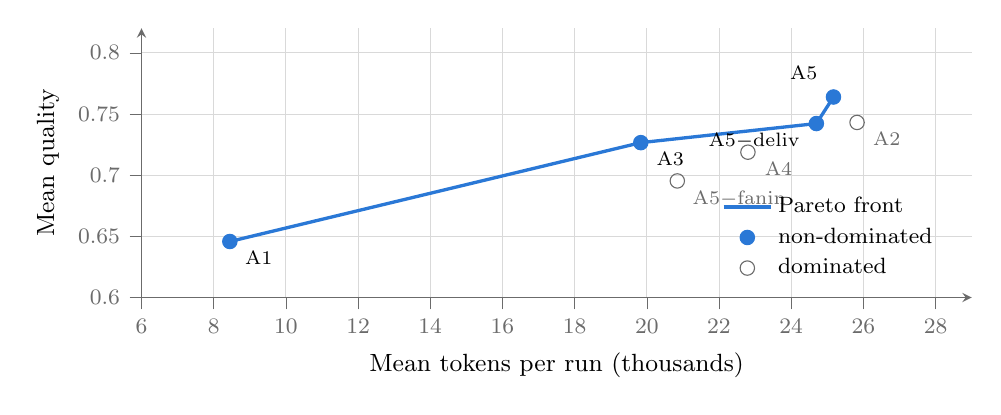
\begin{tikzpicture}
\begin{axis}[paperaxis,
  xlabel={Mean tokens per run (thousands)},
  ylabel={Mean quality},
  xmin=6, xmax=29, ymin=0.60, ymax=0.82,
  ytick={0.60,0.65,0.70,0.75,0.80},
  legend pos=south east,
]
% 前沿连线先画,置于散点之下。
\addplot[serOne, line width=1.2pt, mark=none] coordinates {
  (8.449,0.6458) (19.834,0.7266) (24.698,0.7422) (25.172,0.7639)
};
\addlegendentry{Pareto front}

% 前沿上的点:实心,蓝。
\addplot[only marks, mark=*, mark size=2.6pt, serOne] coordinates {
  (8.449,0.6458) (19.834,0.7266) (24.698,0.7422) (25.172,0.7639)
};
\addlegendentry{non-dominated}

% 被支配的点:空心,灰 —— 身份不靠颜色单独承担,形状也不同。
\addplot[only marks, mark=o, mark size=2.6pt, inkMuted] coordinates {
  (25.825,0.7431) (22.802,0.7188) (20.845,0.6953)
};
\addlegendentry{dominated}

% 直接标注(对比度 WARN 要求可见标签;论文图本应如此)。
\node[font=\scriptsize, anchor=north west] at (axis cs:8.6,0.6458) {A1};
\node[font=\scriptsize, anchor=north west] at (axis cs:20.0,0.7266) {A3};
\node[font=\scriptsize, anchor=north east] at (axis cs:24.5,0.7422) {A5$-$deliv};
\node[font=\scriptsize, anchor=south east] at (axis cs:25.0,0.7700) {A5};
\node[font=\scriptsize, anchor=north west, inkMuted] at (axis cs:26.0,0.7431) {A2};
\node[font=\scriptsize, anchor=north west, inkMuted] at (axis cs:23.0,0.7188) {A4};
\node[font=\scriptsize, anchor=north west, inkMuted] at (axis cs:21.0,0.6953) {A5$-$fanin};
\end{axis}
\end{tikzpicture}
\caption{Quality against cost. Four conditions are non-dominated, so no arm is
simply better --- this is a genuine trade-off, which is why we treat the front
as the primary result and the scalarised objective $R$ as a summary. A1 buys
$0.646$ quality for $8.4$k tokens; reaching $0.764$ costs three times that.}
\label{fig:pareto}
\end{figure}

% ── 图 2:条件性效应(强调式)────────────────────────────────────────────────
\begin{figure}[t]
\centering
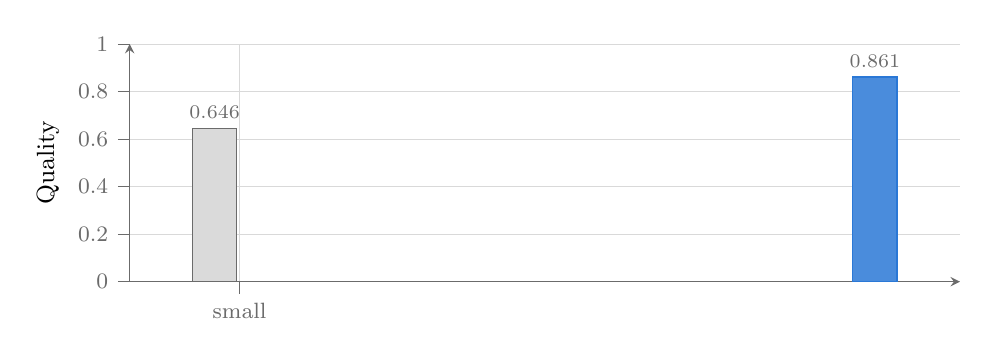
\begin{tikzpicture}
\begin{axis}[paperaxis, height=4.6cm,
  ybar, bar width=16pt,
  symbolic x coords={small, mid, spawned, not spawned},
  xtick=data,
  ylabel={Quality},
  ymin=0, ymax=1.0,
  ytick={0,0.2,0.4,0.6,0.8,1.0},
  nodes near coords, nodes near coords style={font=\scriptsize, color=inkMuted},
  point meta=explicit symbolic,
  enlarge x limits=0.18,
]
% 强调:有效应的条件着色,无效应的灰化。任务是"效应何时存在",
% 不是"比较四个类别",故用单色+灰而非四个类别色。
\addplot[fill=inkMuted!25, draw=inkMuted, line width=0.5pt] coordinates {
  (small,0.6458) [0.646]
};
\addplot[fill=serOne!85, draw=serOne, line width=0.5pt] coordinates {
  (mid,0.8611) [0.861]
};
\end{axis}
\end{tikzpicture}

\vspace{-0.4em}
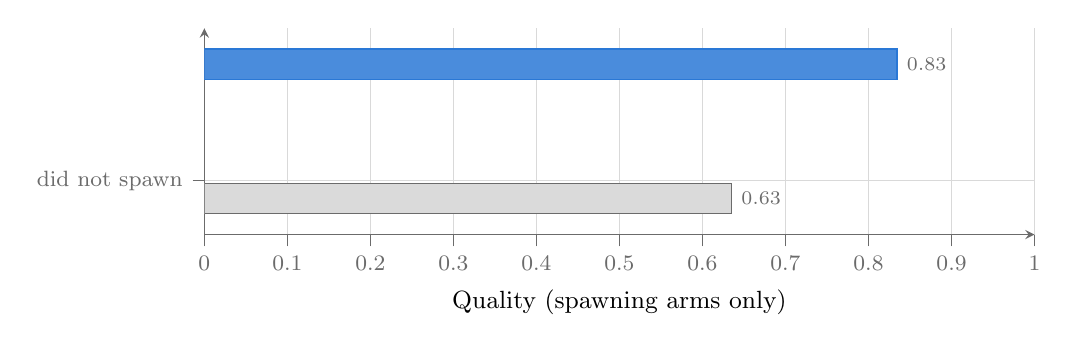
\begin{tikzpicture}
\begin{axis}[paperaxis, height=4.2cm,
  xbar, bar width=11pt,
  symbolic y coords={{did not spawn},{spawned}},
  ytick=data,
  xlabel={Quality (spawning arms only)},
  xmin=0, xmax=1.0,
  nodes near coords, nodes near coords style={font=\scriptsize, color=inkMuted},
  enlarge y limits=0.55,
]
\addplot[fill=inkMuted!25, draw=inkMuted, line width=0.5pt]
  coordinates {(0.6348,{did not spawn})};
\addplot[fill=serOne!85, draw=serOne, line width=0.5pt]
  coordinates {(0.8342,{spawned})};
\end{axis}
\end{tikzpicture}
\caption{The effect is conditional on the orchestrator actually decomposing.
\emph{Top}: A5 quality by tier --- the small tier, whose orchestrators declined
to delegate in 94\% of eligible cells, is shaded out because no arm beat the
baseline there. \emph{Bottom}: regrouping spawning-arm cells by behaviour rather
than tier. The $0.199$ gap between cells that spawned and cells that did not
exceeds any difference we measured between arms.}
\label{fig:conditional}
\end{figure}

% ── 图 3:配对差值与置信区间(forest plot)──────────────────────────────────
\begin{figure}[t]
\centering
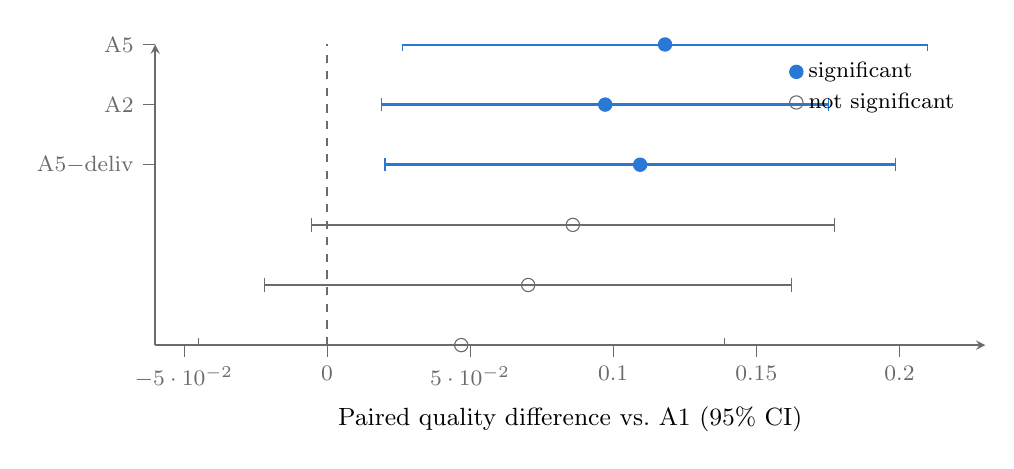
\begin{tikzpicture}
\begin{axis}[paperaxis, height=5.4cm,
  xlabel={Paired quality difference vs.\ A1 (95\% CI)},
  symbolic y coords={{A5$-$fanin},{A4},{A3},{A5$-$deliv},{A2},{A5}},
  ytick=data,
  xmin=-0.06, xmax=0.23,
  xtick={-0.05,0,0.05,0.10,0.15,0.20},
  grid=none,
]
% 零线是判据,画成最显眼的参考线。
\draw[inkMuted, line width=0.8pt, dashed]
  (axis cs:0,{A5$-$fanin}) -- (axis cs:0,{A5});

% 显著(区间不含 0):蓝、实心。
\addplot[only marks, mark=*, mark size=2.4pt, serOne,
  error bars/.cd, x dir=both, x explicit, error bar style={serOne, line width=0.9pt}]
  coordinates {
    (0.1181,{A5})        +- (0.0918,0)
    (0.0972,{A2})        +- (0.0781,0)
    (0.1094,{A5$-$deliv}) +- (0.0891,0)
  };
\addlegendentry{significant}

% 不显著:灰、空心 —— 形状与颜色双编码。
\addplot[only marks, mark=o, mark size=2.4pt, inkMuted,
  error bars/.cd, x dir=both, x explicit, error bar style={inkMuted, line width=0.9pt}]
  coordinates {
    (0.0859,{A3})          +- (0.0914,0)
    (0.0703,{A4})          +- (0.0921,0)
    (0.0469,{A5$-$fanin})  +- (0.0919,0)
  };
\addlegendentry{not significant}
\end{axis}
\end{tikzpicture}
\caption{Paired per-instance differences against the single-agent baseline, each
on the same task, seed and model. Every point is positive, but three intervals
cross zero. The informative contrast is A5 ($+0.118$) against A5 with fan-in
disabled ($+0.047$, interval spanning zero): removing declarative data flow
collapses the effect, while removing relevance-routed delivery
(A5$-$deliv, $+0.109$) barely moves it.}
\label{fig:paired}
\end{figure}

% ── 图 4:λ 扫描下的排名翻转 ────────────────────────────────────────────────
\begin{figure}[t]
\centering
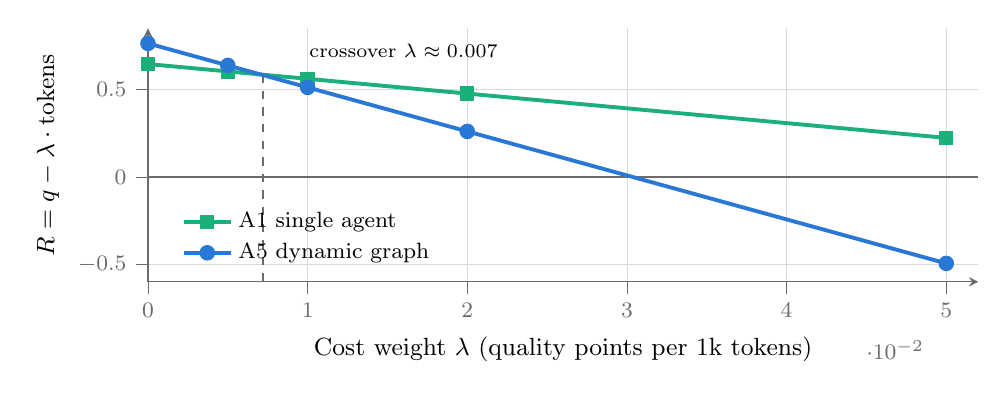
\begin{tikzpicture}
\begin{axis}[paperaxis, height=4.8cm,
  xlabel={Cost weight $\lambda$ (quality points per 1k tokens)},
  ylabel={$R = q - \lambda \cdot \mathrm{tokens}$},
  xmin=0, xmax=0.052,
  ymin=-0.6, ymax=0.85,
  xtick={0,0.01,0.02,0.03,0.04,0.05},
  legend pos=south west,
]
\draw[inkMuted, line width=0.5pt] (axis cs:0,0) -- (axis cs:0.052,0);

\addplot[serTwo, line width=1.4pt, mark=square*, mark size=1.9pt] coordinates {
  (0,0.6458) (0.005,0.6036) (0.01,0.5613) (0.02,0.4769) (0.05,0.2234)
};
\addlegendentry{A1 single agent}

\addplot[serOne, line width=1.4pt, mark=*, mark size=2.1pt] coordinates {
  (0,0.7639) (0.005,0.6380) (0.01,0.5122) (0.02,0.2604) (0.05,-0.4947)
};
\addlegendentry{A5 dynamic graph}

% 交点标注:这是本图唯一要传达的结论。
\draw[inkMuted, dashed, line width=0.5pt]
  (axis cs:0.0072,-0.6) -- (axis cs:0.0072,0.58);
\node[font=\scriptsize, anchor=west, align=left] at (axis cs:0.0095,0.72)
  {crossover $\lambda \approx 0.007$};
\end{axis}
\end{tikzpicture}
\caption{Ranking under the scalarised objective flips almost immediately. With
cost unweighted A5 leads by $0.118$; by $\lambda \approx 0.007$ --- seven
thousandths of a quality point per thousand tokens --- the single-agent baseline
overtakes it and stays ahead. No defensible argument picks a single $\lambda$,
which is why Figure~\ref{fig:pareto} rather than $R$ carries the result.}
\label{fig:sweep}
\end{figure}
 引入。
%
% ## 形式选择的依据(每图一个"读者要做什么")
%
% 1. Pareto 前沿 → 散点 + 前沿连线。任务是"在二维权衡里找非被支配点",
%    这是散点唯一胜过柱状图的场合;前沿连线把"被支配"变成视觉可判。
% 2. 条件性效应 → 强调式(emphasis)柱状对比。任务不是"比较两档",而是
%    "看一个效应在何条件下存在",故一档着色、另一档灰化,而非两个同权重的类别色。
% 3. 配对差值 → 带置信区间的点线图(forest plot)。任务是"哪些差值跨过 0",
%    零线是判据,故零线必须是图上最显眼的参考线。
% 4. λ 扫描交叉 → 双线折线。任务是"排名在何处翻转",交点即答案。
%
% ## 颜色
%
% 取 dataviz 参考调色板的分类槽位,并已跑验证器:
%   CVD 最差相邻对 ΔE 24.2(protan)/ 21.6(tritan),远高于 12 的目标线;
%   对比度检查给出 WARN(低于 3:1),据此**所有系列一律直接标注**——
%   论文图本就该直接标注,故该约束不增成本。
% 单色+灰的强调式用于图 2:那里的任务是突出一个条件,不是区分两个类别。

\definecolor{serOne}{HTML}{2A78D6}   % 蓝:主系列 / 前沿
\definecolor{serTwo}{HTML}{1BAF7A}   % 青:对照系列
\definecolor{serThree}{HTML}{EDA100} % 黄
\definecolor{inkMuted}{HTML}{6B6B6B} % 去强调灰
\definecolor{inkGrid}{HTML}{D9D9D9}  % 网格(退让)

% 所有图共用的退让式坐标轴样式:细线、浅网格、无顶右框。
\pgfplotsset{
  paperaxis/.style={
    width=\linewidth, height=5.0cm,
    axis lines=left,
    axis line style={inkMuted, line width=0.5pt},
    tick label style={font=\footnotesize, color=inkMuted},
    label style={font=\small},
    title style={font=\small, align=left},
    grid=major,
    grid style={inkGrid, line width=0.3pt},
    tick align=outside, tick style={inkMuted},
    legend cell align=left,
    legend style={font=\footnotesize, draw=none, fill=none},
  },
}

% ── 图 1:质量—成本 Pareto 前沿 ──────────────────────────────────────────────
\begin{figure}[t]
\centering
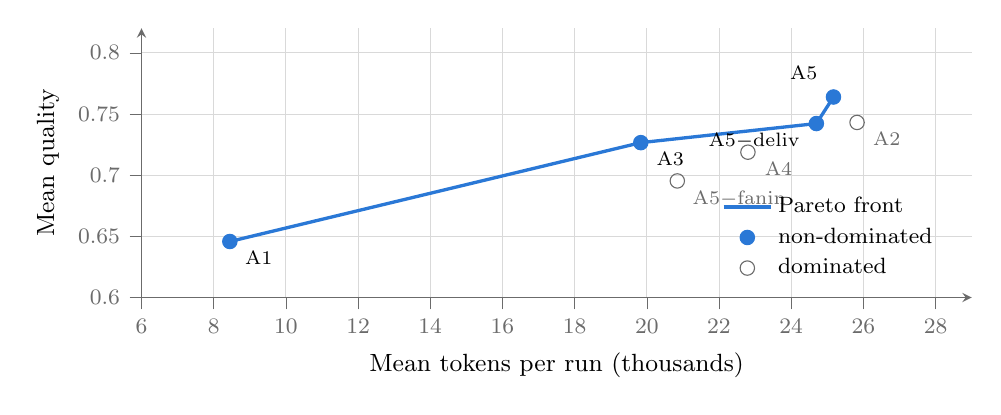
\begin{tikzpicture}
\begin{axis}[paperaxis,
  xlabel={Mean tokens per run (thousands)},
  ylabel={Mean quality},
  xmin=6, xmax=29, ymin=0.60, ymax=0.82,
  ytick={0.60,0.65,0.70,0.75,0.80},
  legend pos=south east,
]
% 前沿连线先画,置于散点之下。
\addplot[serOne, line width=1.2pt, mark=none] coordinates {
  (8.449,0.6458) (19.834,0.7266) (24.698,0.7422) (25.172,0.7639)
};
\addlegendentry{Pareto front}

% 前沿上的点:实心,蓝。
\addplot[only marks, mark=*, mark size=2.6pt, serOne] coordinates {
  (8.449,0.6458) (19.834,0.7266) (24.698,0.7422) (25.172,0.7639)
};
\addlegendentry{non-dominated}

% 被支配的点:空心,灰 —— 身份不靠颜色单独承担,形状也不同。
\addplot[only marks, mark=o, mark size=2.6pt, inkMuted] coordinates {
  (25.825,0.7431) (22.802,0.7188) (20.845,0.6953)
};
\addlegendentry{dominated}

% 直接标注(对比度 WARN 要求可见标签;论文图本应如此)。
\node[font=\scriptsize, anchor=north west] at (axis cs:8.6,0.6458) {A1};
\node[font=\scriptsize, anchor=north west] at (axis cs:20.0,0.7266) {A3};
\node[font=\scriptsize, anchor=north east] at (axis cs:24.5,0.7422) {A5$-$deliv};
\node[font=\scriptsize, anchor=south east] at (axis cs:25.0,0.7700) {A5};
\node[font=\scriptsize, anchor=north west, inkMuted] at (axis cs:26.0,0.7431) {A2};
\node[font=\scriptsize, anchor=north west, inkMuted] at (axis cs:23.0,0.7188) {A4};
\node[font=\scriptsize, anchor=north west, inkMuted] at (axis cs:21.0,0.6953) {A5$-$fanin};
\end{axis}
\end{tikzpicture}
\caption{Quality against cost. Four conditions are non-dominated, so no arm is
simply better --- this is a genuine trade-off, which is why we treat the front
as the primary result and the scalarised objective $R$ as a summary. A1 buys
$0.646$ quality for $8.4$k tokens; reaching $0.764$ costs three times that.}
\label{fig:pareto}
\end{figure}

% ── 图 2:条件性效应(强调式)────────────────────────────────────────────────
\begin{figure}[t]
\centering
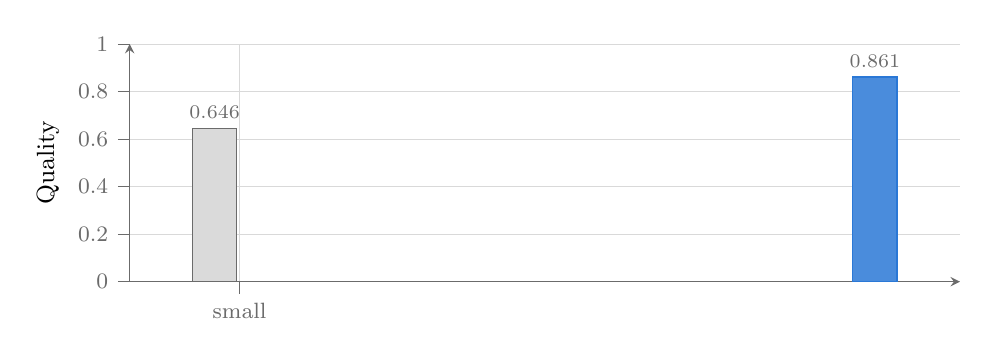
\begin{tikzpicture}
\begin{axis}[paperaxis, height=4.6cm,
  ybar, bar width=16pt,
  symbolic x coords={small, mid, spawned, not spawned},
  xtick=data,
  ylabel={Quality},
  ymin=0, ymax=1.0,
  ytick={0,0.2,0.4,0.6,0.8,1.0},
  nodes near coords, nodes near coords style={font=\scriptsize, color=inkMuted},
  point meta=explicit symbolic,
  enlarge x limits=0.18,
]
% 强调:有效应的条件着色,无效应的灰化。任务是"效应何时存在",
% 不是"比较四个类别",故用单色+灰而非四个类别色。
\addplot[fill=inkMuted!25, draw=inkMuted, line width=0.5pt] coordinates {
  (small,0.6458) [0.646]
};
\addplot[fill=serOne!85, draw=serOne, line width=0.5pt] coordinates {
  (mid,0.8611) [0.861]
};
\end{axis}
\end{tikzpicture}

\vspace{-0.4em}
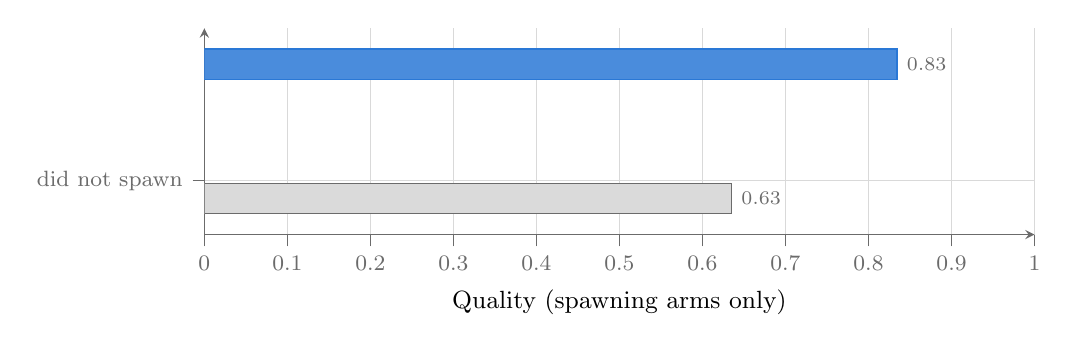
\begin{tikzpicture}
\begin{axis}[paperaxis, height=4.2cm,
  xbar, bar width=11pt,
  symbolic y coords={{did not spawn},{spawned}},
  ytick=data,
  xlabel={Quality (spawning arms only)},
  xmin=0, xmax=1.0,
  nodes near coords, nodes near coords style={font=\scriptsize, color=inkMuted},
  enlarge y limits=0.55,
]
\addplot[fill=inkMuted!25, draw=inkMuted, line width=0.5pt]
  coordinates {(0.6348,{did not spawn})};
\addplot[fill=serOne!85, draw=serOne, line width=0.5pt]
  coordinates {(0.8342,{spawned})};
\end{axis}
\end{tikzpicture}
\caption{The effect is conditional on the orchestrator actually decomposing.
\emph{Top}: A5 quality by tier --- the small tier, whose orchestrators declined
to delegate in 94\% of eligible cells, is shaded out because no arm beat the
baseline there. \emph{Bottom}: regrouping spawning-arm cells by behaviour rather
than tier. The $0.199$ gap between cells that spawned and cells that did not
exceeds any difference we measured between arms.}
\label{fig:conditional}
\end{figure}

% ── 图 3:配对差值与置信区间(forest plot)──────────────────────────────────
\begin{figure}[t]
\centering
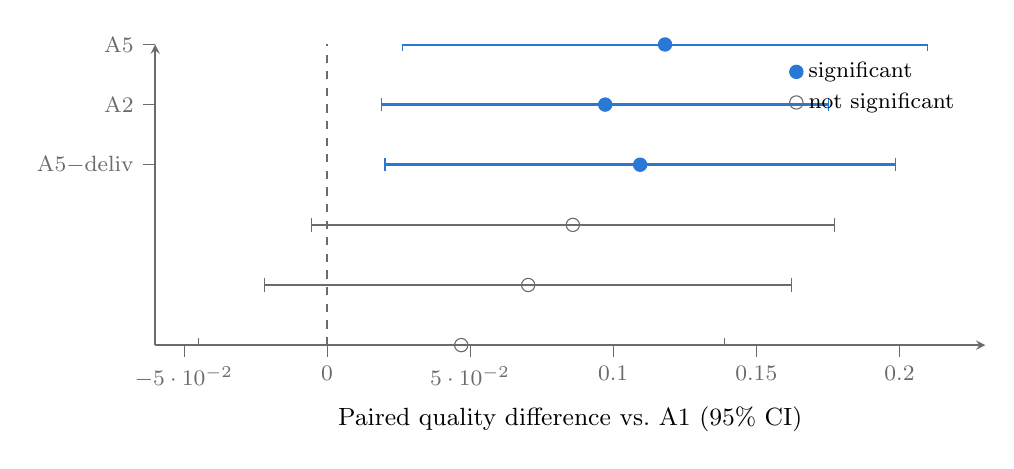
\begin{tikzpicture}
\begin{axis}[paperaxis, height=5.4cm,
  xlabel={Paired quality difference vs.\ A1 (95\% CI)},
  symbolic y coords={{A5$-$fanin},{A4},{A3},{A5$-$deliv},{A2},{A5}},
  ytick=data,
  xmin=-0.06, xmax=0.23,
  xtick={-0.05,0,0.05,0.10,0.15,0.20},
  grid=none,
]
% 零线是判据,画成最显眼的参考线。
\draw[inkMuted, line width=0.8pt, dashed]
  (axis cs:0,{A5$-$fanin}) -- (axis cs:0,{A5});

% 显著(区间不含 0):蓝、实心。
\addplot[only marks, mark=*, mark size=2.4pt, serOne,
  error bars/.cd, x dir=both, x explicit, error bar style={serOne, line width=0.9pt}]
  coordinates {
    (0.1181,{A5})        +- (0.0918,0)
    (0.0972,{A2})        +- (0.0781,0)
    (0.1094,{A5$-$deliv}) +- (0.0891,0)
  };
\addlegendentry{significant}

% 不显著:灰、空心 —— 形状与颜色双编码。
\addplot[only marks, mark=o, mark size=2.4pt, inkMuted,
  error bars/.cd, x dir=both, x explicit, error bar style={inkMuted, line width=0.9pt}]
  coordinates {
    (0.0859,{A3})          +- (0.0914,0)
    (0.0703,{A4})          +- (0.0921,0)
    (0.0469,{A5$-$fanin})  +- (0.0919,0)
  };
\addlegendentry{not significant}
\end{axis}
\end{tikzpicture}
\caption{Paired per-instance differences against the single-agent baseline, each
on the same task, seed and model. Every point is positive, but three intervals
cross zero. The informative contrast is A5 ($+0.118$) against A5 with fan-in
disabled ($+0.047$, interval spanning zero): removing declarative data flow
collapses the effect, while removing relevance-routed delivery
(A5$-$deliv, $+0.109$) barely moves it.}
\label{fig:paired}
\end{figure}

% ── 图 4:λ 扫描下的排名翻转 ────────────────────────────────────────────────
\begin{figure}[t]
\centering
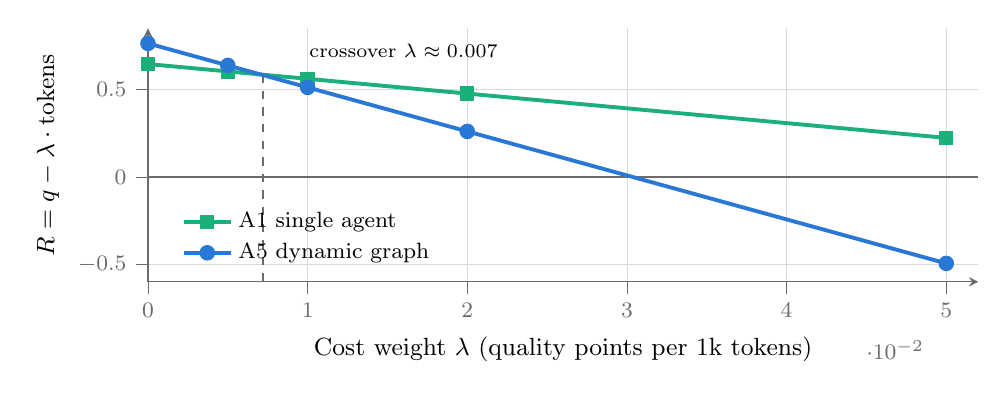
\begin{tikzpicture}
\begin{axis}[paperaxis, height=4.8cm,
  xlabel={Cost weight $\lambda$ (quality points per 1k tokens)},
  ylabel={$R = q - \lambda \cdot \mathrm{tokens}$},
  xmin=0, xmax=0.052,
  ymin=-0.6, ymax=0.85,
  xtick={0,0.01,0.02,0.03,0.04,0.05},
  legend pos=south west,
]
\draw[inkMuted, line width=0.5pt] (axis cs:0,0) -- (axis cs:0.052,0);

\addplot[serTwo, line width=1.4pt, mark=square*, mark size=1.9pt] coordinates {
  (0,0.6458) (0.005,0.6036) (0.01,0.5613) (0.02,0.4769) (0.05,0.2234)
};
\addlegendentry{A1 single agent}

\addplot[serOne, line width=1.4pt, mark=*, mark size=2.1pt] coordinates {
  (0,0.7639) (0.005,0.6380) (0.01,0.5122) (0.02,0.2604) (0.05,-0.4947)
};
\addlegendentry{A5 dynamic graph}

% 交点标注:这是本图唯一要传达的结论。
\draw[inkMuted, dashed, line width=0.5pt]
  (axis cs:0.0072,-0.6) -- (axis cs:0.0072,0.58);
\node[font=\scriptsize, anchor=west, align=left] at (axis cs:0.0095,0.72)
  {crossover $\lambda \approx 0.007$};
\end{axis}
\end{tikzpicture}
\caption{Ranking under the scalarised objective flips almost immediately. With
cost unweighted A5 leads by $0.118$; by $\lambda \approx 0.007$ --- seven
thousandths of a quality point per thousand tokens --- the single-agent baseline
overtakes it and stays ahead. No defensible argument picks a single $\lambda$,
which is why Figure~\ref{fig:pareto} rather than $R$ carries the result.}
\label{fig:sweep}
\end{figure}
 引入。
%
% ## 形式选择的依据(每图一个"读者要做什么")
%
% 1. Pareto 前沿 → 散点 + 前沿连线。任务是"在二维权衡里找非被支配点",
%    这是散点唯一胜过柱状图的场合;前沿连线把"被支配"变成视觉可判。
% 2. 条件性效应 → 强调式(emphasis)柱状对比。任务不是"比较两档",而是
%    "看一个效应在何条件下存在",故一档着色、另一档灰化,而非两个同权重的类别色。
% 3. 配对差值 → 带置信区间的点线图(forest plot)。任务是"哪些差值跨过 0",
%    零线是判据,故零线必须是图上最显眼的参考线。
% 4. λ 扫描交叉 → 双线折线。任务是"排名在何处翻转",交点即答案。
%
% ## 颜色
%
% 取 dataviz 参考调色板的分类槽位,并已跑验证器:
%   CVD 最差相邻对 ΔE 24.2(protan)/ 21.6(tritan),远高于 12 的目标线;
%   对比度检查给出 WARN(低于 3:1),据此**所有系列一律直接标注**——
%   论文图本就该直接标注,故该约束不增成本。
% 单色+灰的强调式用于图 2:那里的任务是突出一个条件,不是区分两个类别。

\definecolor{serOne}{HTML}{2A78D6}   % 蓝:主系列 / 前沿
\definecolor{serTwo}{HTML}{1BAF7A}   % 青:对照系列
\definecolor{serThree}{HTML}{EDA100} % 黄
\definecolor{inkMuted}{HTML}{6B6B6B} % 去强调灰
\definecolor{inkGrid}{HTML}{D9D9D9}  % 网格(退让)

% 所有图共用的退让式坐标轴样式:细线、浅网格、无顶右框。
\pgfplotsset{
  paperaxis/.style={
    width=\linewidth, height=5.0cm,
    axis lines=left,
    axis line style={inkMuted, line width=0.5pt},
    tick label style={font=\footnotesize, color=inkMuted},
    label style={font=\small},
    title style={font=\small, align=left},
    grid=major,
    grid style={inkGrid, line width=0.3pt},
    tick align=outside, tick style={inkMuted},
    legend cell align=left,
    legend style={font=\footnotesize, draw=none, fill=none},
  },
}

% ── 图 1:质量—成本 Pareto 前沿 ──────────────────────────────────────────────
\begin{figure}[t]
\centering
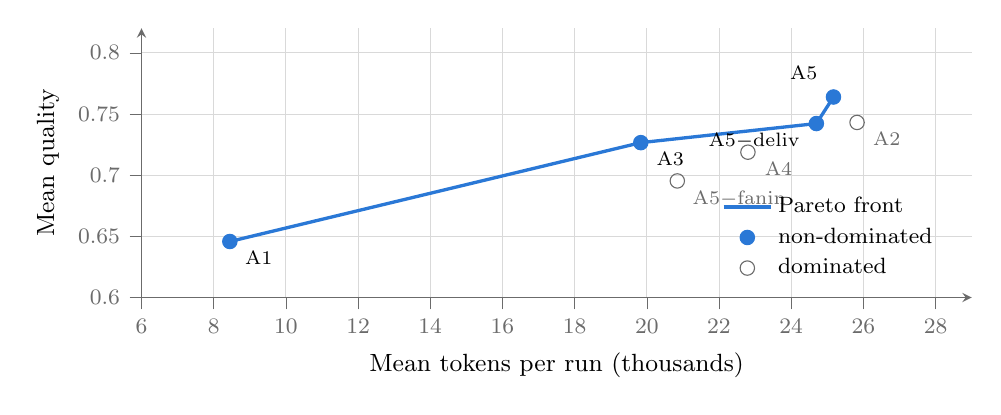
\begin{tikzpicture}
\begin{axis}[paperaxis,
  xlabel={Mean tokens per run (thousands)},
  ylabel={Mean quality},
  xmin=6, xmax=29, ymin=0.60, ymax=0.82,
  ytick={0.60,0.65,0.70,0.75,0.80},
  legend pos=south east,
]
% 前沿连线先画,置于散点之下。
\addplot[serOne, line width=1.2pt, mark=none] coordinates {
  (8.449,0.6458) (19.834,0.7266) (24.698,0.7422) (25.172,0.7639)
};
\addlegendentry{Pareto front}

% 前沿上的点:实心,蓝。
\addplot[only marks, mark=*, mark size=2.6pt, serOne] coordinates {
  (8.449,0.6458) (19.834,0.7266) (24.698,0.7422) (25.172,0.7639)
};
\addlegendentry{non-dominated}

% 被支配的点:空心,灰 —— 身份不靠颜色单独承担,形状也不同。
\addplot[only marks, mark=o, mark size=2.6pt, inkMuted] coordinates {
  (25.825,0.7431) (22.802,0.7188) (20.845,0.6953)
};
\addlegendentry{dominated}

% 直接标注(对比度 WARN 要求可见标签;论文图本应如此)。
\node[font=\scriptsize, anchor=north west] at (axis cs:8.6,0.6458) {A1};
\node[font=\scriptsize, anchor=north west] at (axis cs:20.0,0.7266) {A3};
\node[font=\scriptsize, anchor=north east] at (axis cs:24.5,0.7422) {A5$-$deliv};
\node[font=\scriptsize, anchor=south east] at (axis cs:25.0,0.7700) {A5};
\node[font=\scriptsize, anchor=north west, inkMuted] at (axis cs:26.0,0.7431) {A2};
\node[font=\scriptsize, anchor=north west, inkMuted] at (axis cs:23.0,0.7188) {A4};
\node[font=\scriptsize, anchor=north west, inkMuted] at (axis cs:21.0,0.6953) {A5$-$fanin};
\end{axis}
\end{tikzpicture}
\caption{Quality against cost. Four conditions are non-dominated, so no arm is
simply better --- this is a genuine trade-off, which is why we treat the front
as the primary result and the scalarised objective $R$ as a summary. A1 buys
$0.646$ quality for $8.4$k tokens; reaching $0.764$ costs three times that.}
\label{fig:pareto}
\end{figure}

% ── 图 2:条件性效应(强调式)────────────────────────────────────────────────
\begin{figure}[t]
\centering
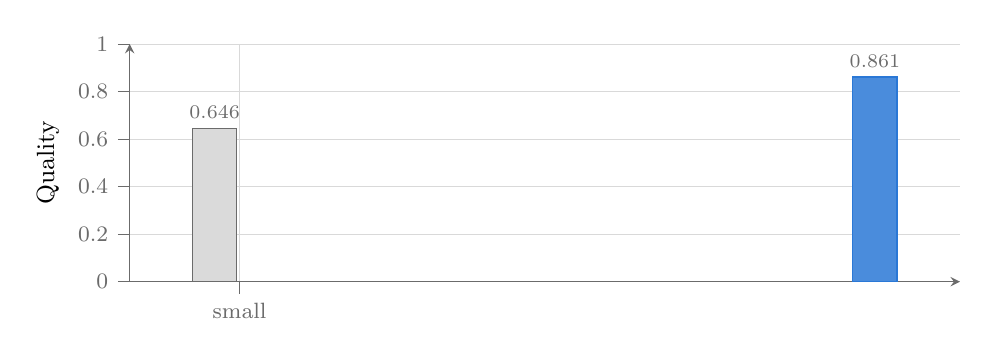
\begin{tikzpicture}
\begin{axis}[paperaxis, height=4.6cm,
  ybar, bar width=16pt,
  symbolic x coords={small, mid, spawned, not spawned},
  xtick=data,
  ylabel={Quality},
  ymin=0, ymax=1.0,
  ytick={0,0.2,0.4,0.6,0.8,1.0},
  nodes near coords, nodes near coords style={font=\scriptsize, color=inkMuted},
  point meta=explicit symbolic,
  enlarge x limits=0.18,
]
% 强调:有效应的条件着色,无效应的灰化。任务是"效应何时存在",
% 不是"比较四个类别",故用单色+灰而非四个类别色。
\addplot[fill=inkMuted!25, draw=inkMuted, line width=0.5pt] coordinates {
  (small,0.6458) [0.646]
};
\addplot[fill=serOne!85, draw=serOne, line width=0.5pt] coordinates {
  (mid,0.8611) [0.861]
};
\end{axis}
\end{tikzpicture}

\vspace{-0.4em}
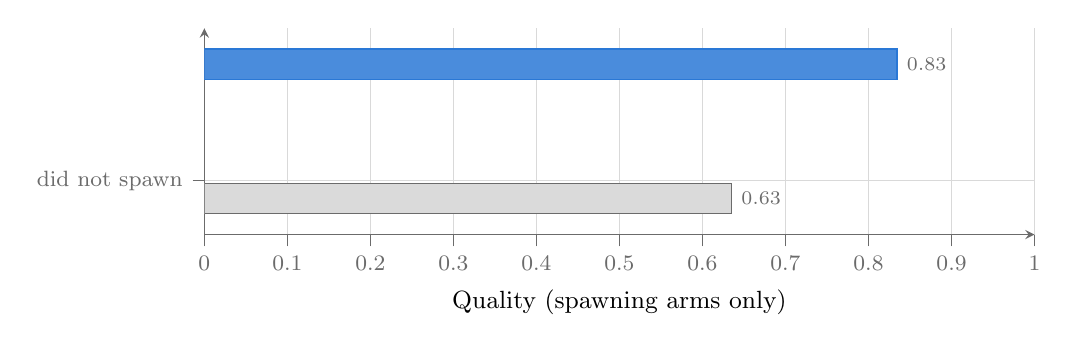
\begin{tikzpicture}
\begin{axis}[paperaxis, height=4.2cm,
  xbar, bar width=11pt,
  symbolic y coords={{did not spawn},{spawned}},
  ytick=data,
  xlabel={Quality (spawning arms only)},
  xmin=0, xmax=1.0,
  nodes near coords, nodes near coords style={font=\scriptsize, color=inkMuted},
  enlarge y limits=0.55,
]
\addplot[fill=inkMuted!25, draw=inkMuted, line width=0.5pt]
  coordinates {(0.6348,{did not spawn})};
\addplot[fill=serOne!85, draw=serOne, line width=0.5pt]
  coordinates {(0.8342,{spawned})};
\end{axis}
\end{tikzpicture}
\caption{The effect is conditional on the orchestrator actually decomposing.
\emph{Top}: A5 quality by tier --- the small tier, whose orchestrators declined
to delegate in 94\% of eligible cells, is shaded out because no arm beat the
baseline there. \emph{Bottom}: regrouping spawning-arm cells by behaviour rather
than tier. The $0.199$ gap between cells that spawned and cells that did not
exceeds any difference we measured between arms.}
\label{fig:conditional}
\end{figure}

% ── 图 3:配对差值与置信区间(forest plot)──────────────────────────────────
\begin{figure}[t]
\centering
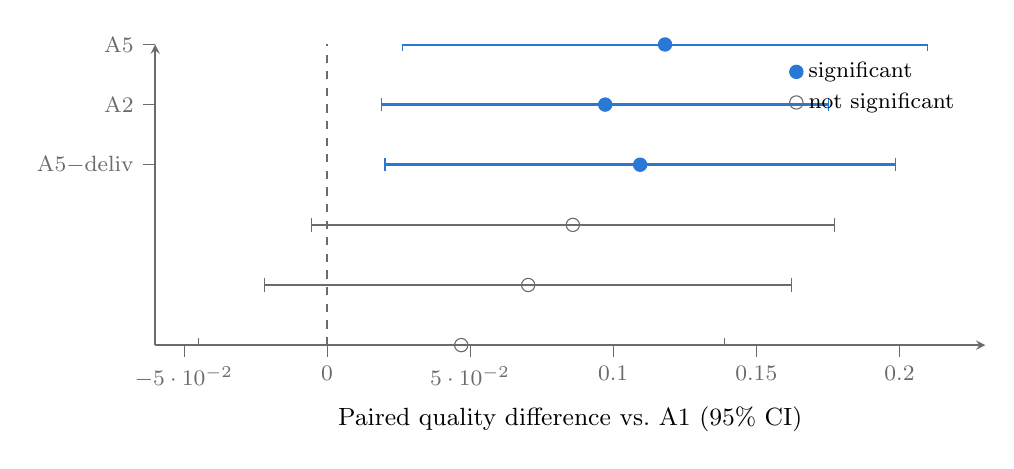
\begin{tikzpicture}
\begin{axis}[paperaxis, height=5.4cm,
  xlabel={Paired quality difference vs.\ A1 (95\% CI)},
  symbolic y coords={{A5$-$fanin},{A4},{A3},{A5$-$deliv},{A2},{A5}},
  ytick=data,
  xmin=-0.06, xmax=0.23,
  xtick={-0.05,0,0.05,0.10,0.15,0.20},
  grid=none,
]
% 零线是判据,画成最显眼的参考线。
\draw[inkMuted, line width=0.8pt, dashed]
  (axis cs:0,{A5$-$fanin}) -- (axis cs:0,{A5});

% 显著(区间不含 0):蓝、实心。
\addplot[only marks, mark=*, mark size=2.4pt, serOne,
  error bars/.cd, x dir=both, x explicit, error bar style={serOne, line width=0.9pt}]
  coordinates {
    (0.1181,{A5})        +- (0.0918,0)
    (0.0972,{A2})        +- (0.0781,0)
    (0.1094,{A5$-$deliv}) +- (0.0891,0)
  };
\addlegendentry{significant}

% 不显著:灰、空心 —— 形状与颜色双编码。
\addplot[only marks, mark=o, mark size=2.4pt, inkMuted,
  error bars/.cd, x dir=both, x explicit, error bar style={inkMuted, line width=0.9pt}]
  coordinates {
    (0.0859,{A3})          +- (0.0914,0)
    (0.0703,{A4})          +- (0.0921,0)
    (0.0469,{A5$-$fanin})  +- (0.0919,0)
  };
\addlegendentry{not significant}
\end{axis}
\end{tikzpicture}
\caption{Paired per-instance differences against the single-agent baseline, each
on the same task, seed and model. Every point is positive, but three intervals
cross zero. The informative contrast is A5 ($+0.118$) against A5 with fan-in
disabled ($+0.047$, interval spanning zero): removing declarative data flow
collapses the effect, while removing relevance-routed delivery
(A5$-$deliv, $+0.109$) barely moves it.}
\label{fig:paired}
\end{figure}

% ── 图 4:λ 扫描下的排名翻转 ────────────────────────────────────────────────
\begin{figure}[t]
\centering
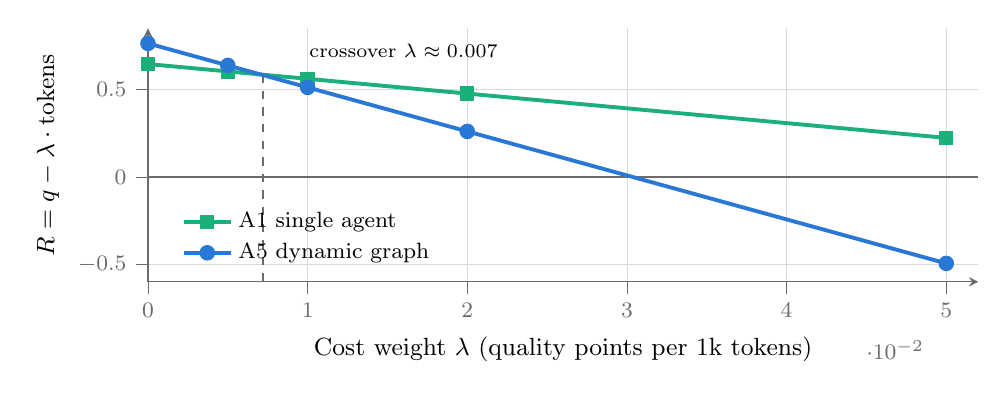
\begin{tikzpicture}
\begin{axis}[paperaxis, height=4.8cm,
  xlabel={Cost weight $\lambda$ (quality points per 1k tokens)},
  ylabel={$R = q - \lambda \cdot \mathrm{tokens}$},
  xmin=0, xmax=0.052,
  ymin=-0.6, ymax=0.85,
  xtick={0,0.01,0.02,0.03,0.04,0.05},
  legend pos=south west,
]
\draw[inkMuted, line width=0.5pt] (axis cs:0,0) -- (axis cs:0.052,0);

\addplot[serTwo, line width=1.4pt, mark=square*, mark size=1.9pt] coordinates {
  (0,0.6458) (0.005,0.6036) (0.01,0.5613) (0.02,0.4769) (0.05,0.2234)
};
\addlegendentry{A1 single agent}

\addplot[serOne, line width=1.4pt, mark=*, mark size=2.1pt] coordinates {
  (0,0.7639) (0.005,0.6380) (0.01,0.5122) (0.02,0.2604) (0.05,-0.4947)
};
\addlegendentry{A5 dynamic graph}

% 交点标注:这是本图唯一要传达的结论。
\draw[inkMuted, dashed, line width=0.5pt]
  (axis cs:0.0072,-0.6) -- (axis cs:0.0072,0.58);
\node[font=\scriptsize, anchor=west, align=left] at (axis cs:0.0095,0.72)
  {crossover $\lambda \approx 0.007$};
\end{axis}
\end{tikzpicture}
\caption{Ranking under the scalarised objective flips almost immediately. With
cost unweighted A5 leads by $0.118$; by $\lambda \approx 0.007$ --- seven
thousandths of a quality point per thousand tokens --- the single-agent baseline
overtakes it and stays ahead. No defensible argument picks a single $\lambda$,
which is why Figure~\ref{fig:pareto} rather than $R$ carries the result.}
\label{fig:sweep}
\end{figure}
 引入。
%
% ## 形式选择的依据(每图一个"读者要做什么")
%
% 1. Pareto 前沿 → 散点 + 前沿连线。任务是"在二维权衡里找非被支配点",
%    这是散点唯一胜过柱状图的场合;前沿连线把"被支配"变成视觉可判。
% 2. 条件性效应 → 强调式(emphasis)柱状对比。任务不是"比较两档",而是
%    "看一个效应在何条件下存在",故一档着色、另一档灰化,而非两个同权重的类别色。
% 3. 配对差值 → 带置信区间的点线图(forest plot)。任务是"哪些差值跨过 0",
%    零线是判据,故零线必须是图上最显眼的参考线。
% 4. λ 扫描交叉 → 双线折线。任务是"排名在何处翻转",交点即答案。
%
% ## 颜色
%
% 取 dataviz 参考调色板的分类槽位,并已跑验证器:
%   CVD 最差相邻对 ΔE 24.2(protan)/ 21.6(tritan),远高于 12 的目标线;
%   对比度检查给出 WARN(低于 3:1),据此**所有系列一律直接标注**——
%   论文图本就该直接标注,故该约束不增成本。
% 单色+灰的强调式用于图 2:那里的任务是突出一个条件,不是区分两个类别。

\definecolor{serOne}{HTML}{2A78D6}   % 蓝:主系列 / 前沿
\definecolor{serTwo}{HTML}{1BAF7A}   % 青:对照系列
\definecolor{serThree}{HTML}{EDA100} % 黄
\definecolor{inkMuted}{HTML}{6B6B6B} % 去强调灰
\definecolor{inkGrid}{HTML}{D9D9D9}  % 网格(退让)

% 所有图共用的退让式坐标轴样式:细线、浅网格、无顶右框。
\pgfplotsset{
  paperaxis/.style={
    width=\linewidth, height=5.0cm,
    axis lines=left,
    axis line style={inkMuted, line width=0.5pt},
    tick label style={font=\footnotesize, color=inkMuted},
    label style={font=\small},
    title style={font=\small, align=left},
    grid=major,
    grid style={inkGrid, line width=0.3pt},
    tick align=outside, tick style={inkMuted},
    legend cell align=left,
    legend style={font=\footnotesize, draw=none, fill=none},
  },
}

